\documentclass[10pt]{beamer}

% template preamble

\usetheme[
	subsectionpage=progressbar, 
	progressbar=frametitle, 
	sectionpage=none, 
	block=fill
]{metropolis}

\usepackage{appendixnumberbeamer}

\usepackage{booktabs}
\usepackage[scale=2]{ccicons}

\usepackage{pgfplots}
\usepgfplotslibrary{dateplot}

\usepackage{xspace}
\newcommand{\themename}{\textbf{\textsc{metropolis}}\xspace}

% eigene packages 
\usepackage[english, ngerman]{babel}
\usepackage{blindtext}
\usepackage{graphicx}

% Macros
\newcommand{\comment}[1]{}



% header
\title{Deep Learning}
\subtitle{Einführung - Thema 2}
\date{\today}
\author{Silas Hoffmann}
\institute{Fachhochschule Wedel}
\titlegraphic{\hfill
\includegraphics[height=1.5cm]{_img/logo_alpha}}

\begin{document}

\maketitle

\begin{frame}
\frametitle{Inhalt}
\tableofcontents
\end{frame}

\part{Geschichtliche Entwicklung}

Im folgenden Abschnitt werde ich etwas auf die geschichtlichen Aspekte von neuronalen Netzen eingehen. Hierbei werden insbesondere die generellen Aspekte der generellen Funktionsweise von älteren Modellen bis hin zur aktuellen Entwicklung verfolgt. Ich werde versuchen die folgenden Leitfragen in diesem Abschnitt zu beantworten: 

\begin{itemize}
\item Woher kommt Deep Learning und wie ist dieser Begriff im Kontext zur künstlichen Intelligenz einzuordnen?
\item Welche Entwicklungen hat das Neuronale Netz von damals zu heute durchgemacht?
\end{itemize}

Um darauf näher eingehen zu können werden folgende Meilensteine behandelt: 

todo Inhaltsverzeichnis (Sections)

\import{geschichtliches/mcCullochPittsNeuron/}{mpNeuron.tex}
\FloatBarrier

\import{geschichtliches/perceptor/}{perceptor.tex}
\FloatBarrier

\import{geschichtliches/adeline/}{adeline.tex}

\section{Aktuelle Entwicklung}

\subsection{Backpropagation}

\begin{frame}
\frametitle{Notation}

\begin{figure}
	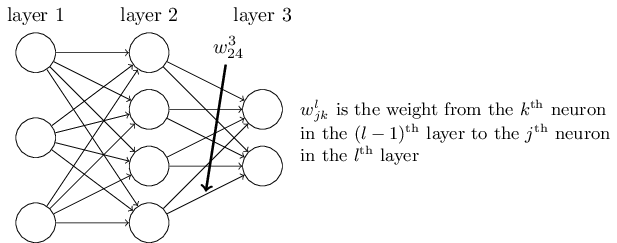
\includegraphics[width=\linewidth]{./aktuelleEntwicklung/backpropagation/img/weight_notation}
\end{figure}

\note[item]{l: Exponent, steht für die Schicht}
\note[item]{l - 1, weil man stets von hinten nach vorne schaut}
\note[item]{Eingabe wird auch als eigene Schicht verstanden}
\note[item]{j: Index Zielneuron}
\note[item]{k: Index Startneuron}

\end{frame}

\begin{frame}
\frametitle{Notation}

\begin{figure}
	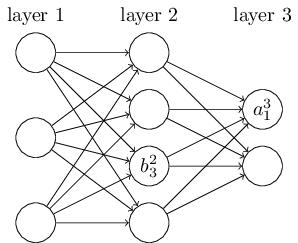
\includegraphics[width=.6\linewidth]{./aktuelleEntwicklung/backpropagation/img/biasAct_notation}
	
\note[item]{Ähnlich zu Gewichtsnotation}
\note[item]{l bezieht sich hierbei jedoch auf aktuelle Schicht}
\note[item]{j wie gehabt Index in Schicht}
\note[item]{Notation gilt auch für Aktivierung a}

\end{figure}

\begin{columns}

\column{.5\textwidth}
\begin{align*}
a^{l}_j = \sigma\left( \sum_k w^{l}_{jk} a^{l-1}_k + b^l_j \right) \Rightarrow 
\quad
\!
\begin{aligned}
a^l & = \sigma(z^l) \\
z^l & = w^l a^{l-1}+b^l \\
\end{aligned}
\end{align*}

\note[item]{Wichtig: $\sigma$ bezieht sich auf Vektor $\Rightarrow$ Vektorielle Funktion}
\note[item]{Jede Komponente einzeln mit $\sigma$ verarbeitet}
\note[item]{Abstraktion vom Ausgabewert vor der Aktivierungsfkt. hilft später beim Ableiten}

\hspace{10mm}

\end{columns}

\end{frame}



\begin{frame}
\frametitle{Backpropagation}

\begin{itemize}
\item{Kostenfunktion soll minimiert werden}
\item{Ziel: Optimale Gewichte und Schwellwerte finden}
\end{itemize}

\begin{itemize}
\item Grobe Vorgehensweise: Iterativer Prozess

\begin{itemize}	
	\item Fehlervektor der letzten Schicht berechnen
	\item Fehler schichtweise zum Eingabelayer zurückführen
	\item Parameter schichtweise nach Gradienten angleichen
\end{itemize}

\end{itemize}


\note[item]{Kostenfunktion wie bei Gradientenabstieg / Adeline}
\note[item]{Unterschied: Hier mehrschichtiges Netz}
\note[item]{1970er entwickelt, 1986 von Rummelhart, Hilten und Williams in Paper bekannt gemacht}
\note[item]{Gradientenabstieg grob erläutert, ausgeblieben - Anwendung im mehrschichtigen Netz und mehrdimensionale Kostenfunktion}

\note[item]{Fehlervektor der letzten Schicht berechnen}
\note[item]{Fehler schichtweise zum Eingabelayer zurückführen}
\note[item]{Parameter schichtweise nach Gradienten angleichen}
\end{frame}


\begin{frame}
\frametitle{Fehler - Ausgabeschicht} 

\begin{columns}

\begin{column}{0.5\textwidth}
\myeq{
\delta^L_j & = \frac{\partial C}{\partial z^L_j} \\
 & = \sum_k \frac{\partial C}{\partial a^L_k} \frac{\partial a^L_k}{\partial z^L_j} \\
 & = \frac{\partial C}{\partial a^L_j} \frac{\partial a^L_j}{\partial z^L_j} \\
 & = \frac{\partial C}{\partial a^L_j} \sigma'(z^L_j)
}

\begin{block}{Anmerkung: Kettenregel}
\myeq{\frac{d}{{dx}}\left[ {f\left( u \right)} \right] = \frac{d}{{du}}\left[ {f\left( u \right)} \right]\frac{{du}}{{dx}}}
\end{block}
\end{column}

\vrule
\vspace{1mm}

\begin{column}{0.5\textwidth}
\vspace{-8mm}

\begin{center}
\begin{forest}
 [C
 	[y]
 	[$a^{L}$
 		[$z^{L}$
			[$w^L$]
			[$a^{L-1}$
				[\ldots]
			]
			[$b^{L}$]
 		]
 	]
 ]
\end{forest}
\end{center}



\begin{itemize}
\item \textbf{C}: Kostenfunktion
\item \textbf{y}: Erwartete Ausgabe
\end{itemize}
\end{column}

\end{columns}

\note[item]{Baum nur für Netz mit einer einzigen Aktivierung}
\note[item]{Zusammenhang mit Kettenregel erläutern}
\note[item]{Großes L immer für Ausgabeschicht}

\end{frame}


\begin{frame}
\frametitle{Fehler - Ausgabeschicht}

\begin{block}{Zusammenfassung}
\begin{itemize}
\item Um den Fehlervektor der letzten Schicht zu bestimmen: 
\myeq{\delta^L = \nabla_a C \odot \sigma'(z^L)}
\item Äquivalent zu: 
\myeq{\delta^L = (a^L-y) \odot \sigma'(z^L)}
\item Um die Fehler komponentenweise zu bestimmen:
\myeq{\delta^L_j = \frac{\partial C}{\partial a^L_j} \sigma'(z^L_j)}
\end{itemize}
\end{block}

\note[item]{$\nabla_a C$ entspricht dabei Vektor aller $\frac{\partial C}{\partial a^L_j}$ einer Schicht}
\note[item]{$\odot$: Komponentenweise Multiplikation zweier Vektoren}

\end{frame}



\begin{frame}
\frametitle{Fehler - Zwischenschicht} 

\begin{itemize}
\item Zusammenhang zwischen Fehler zweier Schichten herleiten
\item Es gilt: $\delta^l_j = \partial C / \partial z^l_j$ sowie $\delta^{l+1}_k = \partial C / \partial z^{l+1}_k$
\end{itemize}

\begin{columns}

\begin{column}{.5\textwidth}
\vspace{-10mm}

\myeq{
\delta^l_j & = \frac{\partial C}{\partial z^l_j} \\
 & = \sum_k \frac{\partial C}{\partial z^{l+1}_k} \frac{\partial z^{l+1}_k}{\partial z^l_j} \\
 & = \sum_k \frac{\partial z^{l+1}_k}{\partial z^l_j} \delta^{l+1}_k
}
\end{column}

\hspace{-15mm}
\vrule

\begin{column}{.5\textwidth}

\begin{center}
\begin{forest}
 [$z^{l+1}$
 	[$w^{l+1}$]
 	[$a^{l}$
 		[$z^{l}$
			[$w^l$]
			[$a^{l-1}$
				[\ldots]
			]
			[$b^{l}$]
 		]
 	]
 	[$b^{l+1}$]
 ]
\end{forest}
\end{center}

\end{column}
\end{columns}

\end{frame}



\begin{frame}
\frametitle{Fehler - Zwischenschicht} 
\vspace{-10mm}

\myeq{
z^{l+1}_k & = \sum_j w^{l+1}_{kj} a^l_j +b^{l+1}_k = \sum_j w^{l+1}_{kj} \sigma(z^l_j) +b^{l+1}_k
}

\vspace{-7mm}

\myeq{
\frac{\partial z^{l+1}_k}{\partial z^l_j} = w^{l+1}_{kj} \sigma'(z^l_j)
}

\begin{block}{Zusammenfassung}
\begin{itemize}
\item Komponentenweise Darstellung: 
\inlineeq{\delta^l_j = \sum_k w^{l+1}_{kj}  \delta^{l+1}_k \sigma'(z^l_j)}
\end{itemize}

\begin{itemize}
\item Vektorielle Darstellung: 
\inlineeq{\delta^l = ((w^{l+1})^T \delta^{l+1}) \odot \sigma'(z^l)}
\end{itemize}

\end{block}
\end{frame}



\begin{frame}
\frametitle{Fehler - Schwellwerte \& Gewichte}

\vspace{-8mm}

\myeq{\scalebox{1.2}{$z^{l}_k = \sum_j w^{l}_{kj} a^{l-1}_j +b^l_k = \sum_j w^l_{kj} \sigma(z^{l-1}_j) +b^l_k$}}

\vspace{3mm}

\begin{columns}
\begin{column}{.5\textwidth}

\begin{block}{Schwellwerte}
\myeq{
\frac{\partial C}{\partial b^l_j} = \frac{\partial C}{\partial z^l_j} \frac{\partial z^l_j}{\partial b^l_j} = \delta^l_j
}
\end{block}

\begin{block}{Gewichte}
\myeq{\frac{\partial C}{\partial w^l_{jk}} = \frac{\partial C}{\partial z^l_j} \frac{\partial z^l_j}{\partial w^l_{jk}} = a^{l-1}_k \delta^l_j
}
\end{block}

\end{column}


\vrule

\begin{column}{.5\textwidth}

\begin{center}
\begin{forest}
 [$z^{l+1}$
 	[$w^{l+1}$]
 	[$a^{l}$
 		[$z^{l}$
			[$w^l$]
			[$a^{l-1}$
				[\ldots]
			]
			[$b^{l}$]
 		]
 	]
 	[$b^{l+1}$]
 ]
\end{forest}
\end{center}

\end{column}
\end{columns}
\end{frame}

\begin{frame}
\frametitle{Anwendung}

\begin{itemize}
\item Menge an Trainingsdatensätzen auswählen
\item Für jeden einzelnen Datensatz: 

\begin{enumerate}
\item \textbf{Feedforward}: Z-Wert und Aktivierung für jede Schicht $l = 2, 3, \ldots, L$ berechnen. 
\begin{itemize}
	\item Z-Wert: $z^{x,l} = w^l a^{l-1}+b^l$
	\item Aktivierung $a^{x,l} = \sigma(z^{l})$
\end{itemize}

\item \textbf{Ausgabe-Fehler} $\delta^{x,L}$: Fehlervektor der Ausgabeschicht berechnen.
\begin{itemize}
	\item $\delta^{L}  = \nabla_a C \odot \sigma'(z^L)$
\end{itemize}

\item \textbf{Backpropagation-Fehler}: Rückwirkend Fehlervektor aller Schichten berechnen.
\begin{itemize}
	\item $\delta^{x,l} = ((w^{l+1})^T \delta^{x,l+1}) \odot \sigma'(z^{x,l})$
\end{itemize}
\end{enumerate}

\item \textbf{Gradientenabstieg}: Gewichte und Schwellwerte getrennt anpassen. 
\begin{itemize}
	\item Gewichte: $w^l \rightarrow w^l-\frac{\eta}{m} \sum_x \delta^{x,l} (a^{x,l-1})^T$
	\item Schwellwerte: $b^l \rightarrow b^l-\frac{\eta}{m} \sum_x \delta^{x,l}$
\end{itemize}


\end{itemize}

\end{frame}
\subsection{convolutionalNN}

\begin{frame}
\frametitle{convolutionalNN}
\blindtext
\end{frame}



\maketitle

\begin{frame}[standout]
Fragen?
\end{frame}

\appendix

\begin{frame}[fragile]{Backup slides}
  Sometimes, it is useful to add slides at the end of your presentation to
  refer to during audience questions.

  The best way to do this is to include the \verb|appendixnumberbeamer|
  package in your preamble and call \verb|\appendix| before your backup slides.

  \themename will automatically turn off slide numbering and progress bars for
  slides in the appendix.
\end{frame}

\begin{frame}[allowframebreaks]{References}
  \nocite{*} 
  \bibliography{../../verweise/verweise}
  \bibliographystyle{abbrv}
\end{frame}


\end{document}